\documentclass[xcolor={dvipsnames}]{beamer}
\usepackage{color, colortbl}
\usepackage[ngerman,english]{babel}
\usepackage[T1]{fontenc}
\usepackage{lmodern}
\usepackage[compatibility=false]{caption}
\usepackage{subcaption}
\usepackage{tikz}
\usepackage{textgreek}
\usepackage{tabularx}
\usepackage{booktabs}
\usepackage{xspace,multicol}
\usepackage{siunitx}
\usepackage{appendixnumberbeamer}
\usepackage[absolute,overlay]{textpos} %for positioning the logos where I want

\usepackage{animate}
\usepackage{multimedia}
\usepackage{fixltx2e}
\usepackage{multicol}
\usepackage{multirow}
\usepackage{comment}
\DeclareSIUnit\year{yr}
\DeclareSIUnit\micron{\micro\metre}
\DeclareSIUnit\mrad{\milli\rad}
\DeclareSIUnit\gauss{G}
\DeclareSIUnit\nb{\nano\barn}
\DeclareSIUnit\pb{\pico\barn}
\DeclareSIUnit\fb{\femto\barn}

\newcommand{\electron}{e$^-$\xspace}
\newcommand{\positron}{e$^+$\xspace}
\newcommand{\murm}{%
  \ifmmode
    \mathchoice
        {\hbox{\normalsize\textmu}}
        {\hbox{\normalsize\textmu}}
        {\hbox{\scriptsize\textmu}}
        {\hbox{\tiny\textmu}}%
  \else
    \textmu
  \fi
}

\mode<presentation>
{
  \usetheme{CambridgeUS}     
  \usecolortheme{lily} 
  \definecolor{beamer@violet}{rgb}{0.5,0.3,0.5} % changed this
  \setbeamercolor{structure}{fg=beamer@violet!70!cyan}
  \setbeamercolor{palette primary}{fg=black, bg=gray!30!white!50!cyan!20!}
  \setbeamercolor{palette secondary}{fg=black, bg=gray!30!white!30!cyan!40!}
  \setbeamercolor*{palette tertiary}{bg=gray!20!white!20!cyan!60!}
  
  \setbeamercolor{frametitle}{fg=cyan!60!white!40!,bg=cyan!80!black}
  \setbeamercolor{title}{fg=cyan!80!black}
  \setbeamercolor{normal text}{fg=black,bg=white}
  \setbeamercolor{alerted text}{fg=beamer@violet}
  \setbeamercolor{example text}{fg=beamer@violet!70!cyan}
  
  \usefonttheme{structureitalicserif} 
  \setbeamertemplate{navigation symbols}{}
  \setbeamertemplate{caption}[numbered]
}
\newcommand{\sidlogo}{
  \setlength{\TPHorizModule}{1pt}
  \setlength{\TPVertModule}{1pt}
   % textblock{}{x,y}: pos(x) = rightUpperCorner + (x * \TPHorizModule), pos(y) = leftUpperCorner - (y * \TPVertModule)
  \begin{textblock}{1}(323,12)
   
\includegraphics[width=40pt,height=26pt]{figures/SiD.jpeg}
  \end{textblock}
  } 
\newcommand{\ilclogo}{
  \setlength{\TPHorizModule}{1pt}
  \setlength{\TPVertModule}{1pt}
   % textblock{}{x,y}: pos(x) = rightUpperCorner + (x * \TPHorizModule), pos(y) = leftUpperCorner - (y * \TPVertModule)
  \begin{textblock}{1}(323,12)
   
\includegraphics[width=40pt,height=26pt]{figures/ILC.jpeg}
  \end{textblock}
} 
\newcommand{\flukalogo}{
  \setlength{\TPHorizModule}{1pt}
  \setlength{\TPVertModule}{1pt}
   % textblock{}{x,y}: pos(x) = rightUpperCorner + (x * \TPHorizModule), pos(y) = leftUpperCorner - (y * \TPVertModule)
  \begin{textblock}{1}(315,12)
   
\includegraphics[width=60pt,height=26pt]{figures/fluka_logo.png}
  \end{textblock}
} 

\title[ILC backgrounds \& SiD Occupancy]{\textbf{\alert{Mini-Workshop on ILC Infrastructure and CFS for Physics and Detectors} \\ \vspace*{0.3cm} \LARGE  Summary of \\Background \& SiD Occupancy Studies}}
\author{\textbf{Anne Sch\"utz}}
\institute{\textbf{DESY}}
\date{\textbf{28. September 2017}}

\titlegraphic{
\includegraphics[height=1.0cm]{figures/ILC.jpeg}\hspace*{6cm}~%
   
\includegraphics[height=1.2cm]{figures/DESY_Logo.png}
}

\begin{document}

{
\usebackgroundtemplate{
 \tikz\node[opacity=0.1]{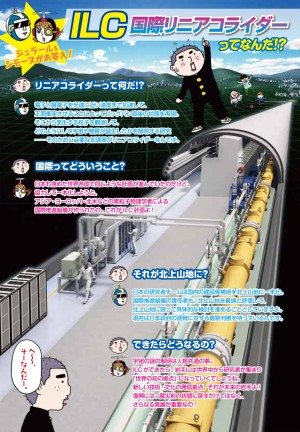
\includegraphics[width=\paperwidth]{figures/Iwatecomics.jpg}};
 % \tikz\node[opacity=0.2]{\centering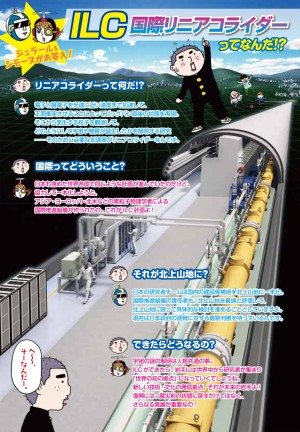
\includegraphics[height=\paperheight]{figures/Iwatecomics.jpg}};
 }
\begin{frame}
  \titlepage
\end{frame}
}

\begin{frame}{Table of contents}
  \tableofcontents
\end{frame}
\begin{frame}{Table of contents}
  For more information, see the more detailed talks:
  \begin{itemize}
   \item BDS muon study:\\
   {\small
   \url{https://agenda.linearcollider.org/event/7371/contributions/38190/attachments/30975/46399/MuonSpoilerStudy_ASchuetz.pdf}
   }
   \item Beam dump study:\\
   {\small
   \url{https://agenda.linearcollider.org/event/7507/contributions/39283/attachments/31735/47826/BeamDump_ASchuetz.pdf}
   }
   \item Pair background study for ILC250 schemes:\\
   {\small
   See LCWS2017 in Strasbourg in October
   }
  \end{itemize}
\end{frame}

%---------------------------------------------------------------------------------------------------------

\section{Muons from the muon spoilers}
\begin{frame}
 \centering \LARGE Muons from the BDS system
\end{frame}

\begin{frame}{BDS tunnel layout}
\ilclogo
\begin{center}
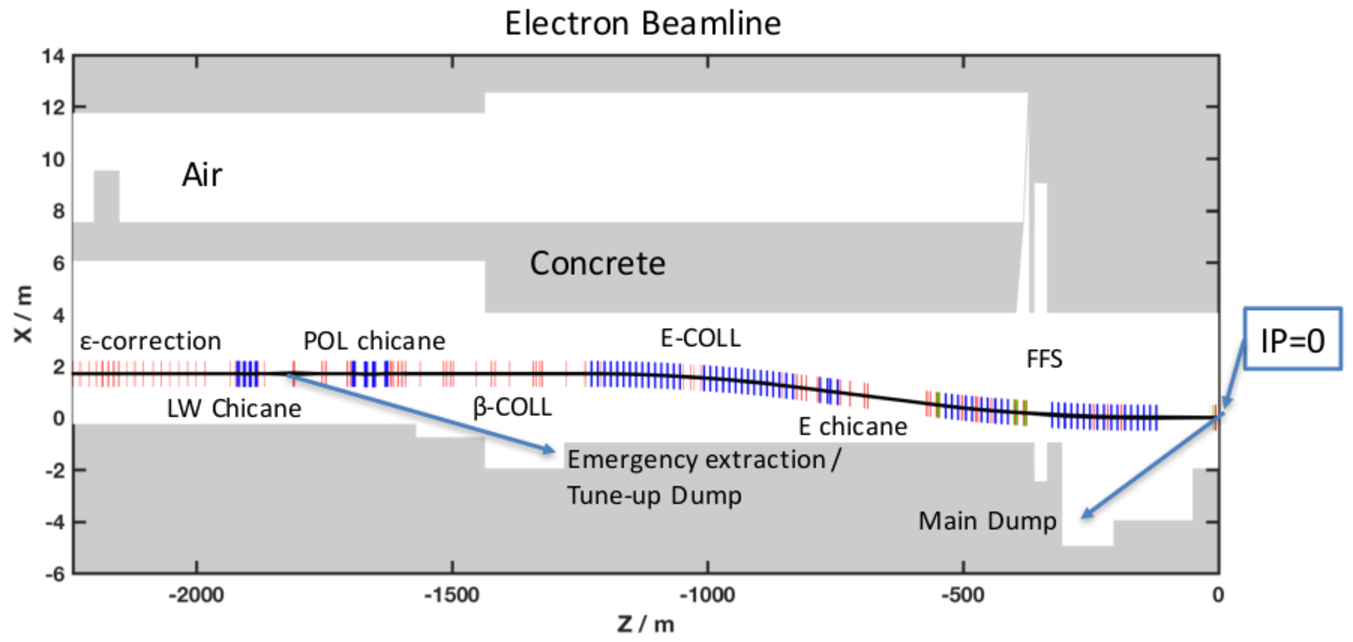
\includegraphics[height=0.65\textheight]{muons_figures/BDS_electron_tunnel.pdf}
\end{center}
\end{frame}

\subsection{Muon spoiler scenarios}
\begin{frame}{Muon spoiler scenarios}
\ilclogo
There are TWO SPOILER SCENARIOS under discussion:
\begin{itemize}
 \item \textbf{5 Spoilers}
 \item \textbf{5 Spoilers + Wall}
\end{itemize}

\begin{columns}[b]
 \begin{column}{0.8\textwidth}
 \flushright
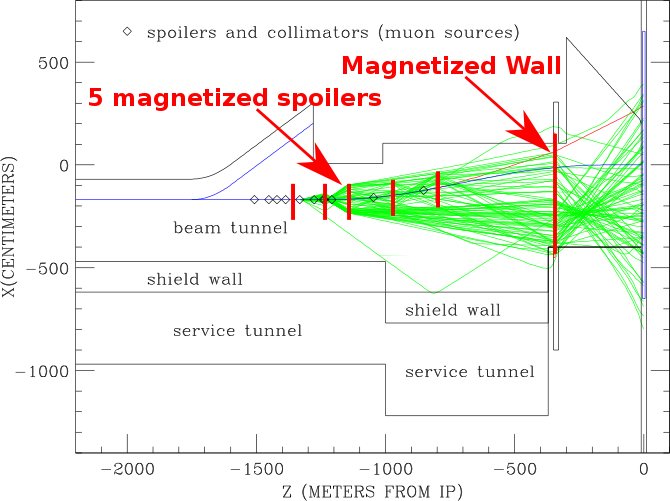
\includegraphics[height=0.67\textheight]{muons_figures/BDS_Tunnel_Spoilers+Wall.png}
\end{column}
 \begin{column}{0.2\textwidth}
 \flushleft
e\textsuperscript{-} beam line
\vspace*{0.55cm}
\end{column}
\end{columns}
\end{frame}

\begin{frame}{5 donut spoilers}
\ilclogo
\textbf{The donut spoilers} are designed as follows:
\begin{itemize}
 \item \SI{70}{\centi\meter} radius
 \item \SI{5}{\meter} long
 \item Magnetized iron with a field of $\sim$10-\SI{19}{\kilo\gauss}
 \item 5 locations (before IP):
 \begin{itemize}
  \item 802.5m
  \item 975.5m
  \item 1145.5m
  \item 1234.5m
  \item 1358.5m
 \end{itemize}

\end{itemize}
\begin{center}
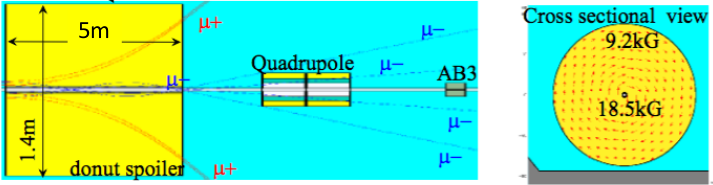
\includegraphics[height=0.3\textheight]{muons_figures/Spoiler.png}
\end{center}
\end{frame}

\begin{frame}{5 donut spoilers + wall}
\ilclogo
\textbf{The iron wall} would completely fill up the tunnel:
\begin{itemize}
 \item \SI{5}{m} x \SI{5}{m}, \SI{5}{m} long
 \item Magnetized with a field of $\sim$\SI{16}{kG}
 \item Located $\sim$\SI{400}{m} away from the IP
 \item Would cost $\sim$ \$3 million
\end{itemize}
\begin{center}
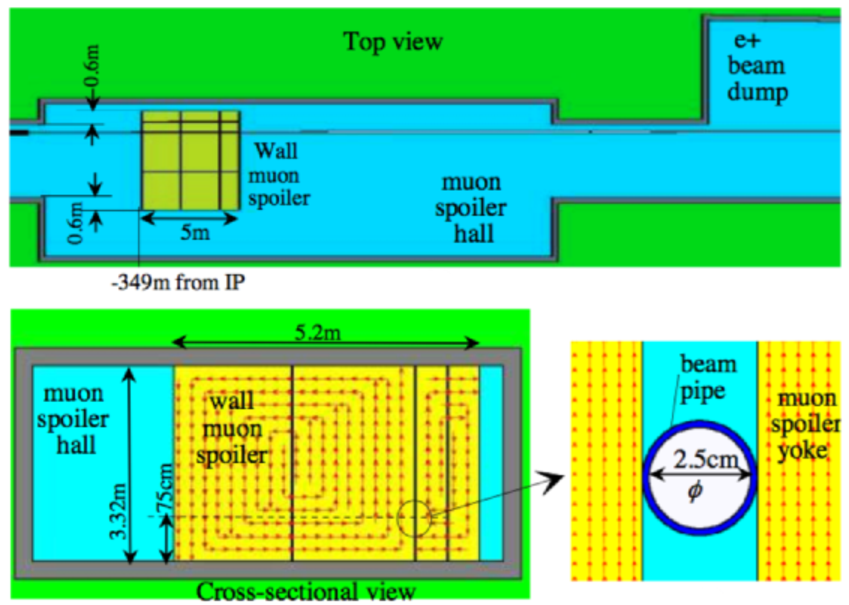
\includegraphics[height=0.7\textheight]{muons_figures/Muon_wall.pdf}
\end{center}
\end{frame}

\section{MUCARLO simulation}
\begin{frame}{MUCARLO simulation overview}
\ilclogo

\begin{columns}
 \begin{column}{0.7\textwidth}
  \begin{itemize}
\item BDS backgrounds with muon collimation system modelled with MUCARLO [Lewis Keller, SLAC] and Geant4 [Glen White, SLAC]
\item Using TDR baseline machine parameters for the ILC500
\item Muon production processes:
\begin{itemize}
\item Predominantly: Bethe-Heitler process:\\ \textgamma + Z $\rightarrow$ Z' + \textmu$^+$\textmu$^-$
\item Few \% level: direct annihilation of positrons with atomic electrons: e$^+$e$^-$ $\rightarrow$ \textmu$^+$\textmu$^-$
\end{itemize}
\item Halo particle tracking:
\begin{itemize}
\item Turtle with MUCARLO
\item Lucretia with a built-in Geant4 model interface
\end{itemize}
\end{itemize}

 \end{column}
 \begin{column}{0.3\textwidth}
  \includegraphics[width=\textwidth]{muons_figures/BetheHeitler.pdf}
 \end{column}
\end{columns}
\end{frame}

\subsection{Muon 4-vectors}
\begin{frame}{Muons in the detector}
\ilclogo
4-vectors of the muons are given to SiD and ILD for studying the effect of the muons on the detector performance.\\
\vspace*{0.2cm}
\begin{tabular}{ll}
\textbf{Scenario} & \textbf{Number of muons in a detector with 6.5m radius}\\
 No Spoilers & 130 muons/bunch crossing\\
 5 Spoilers& 4.3 muons/bunch crossing\\
 5 Spoilers + Wall & 0.6 muons/bunch crossing
\end{tabular}
\end{frame}

\section{Motivation}
\begin{frame}{}
Question to SiD and ILD: Do we need the muon wall at all?!
MID people would be happy to get rid of it because of safety issues, and the costs for such a iron wall.
\begin{center}
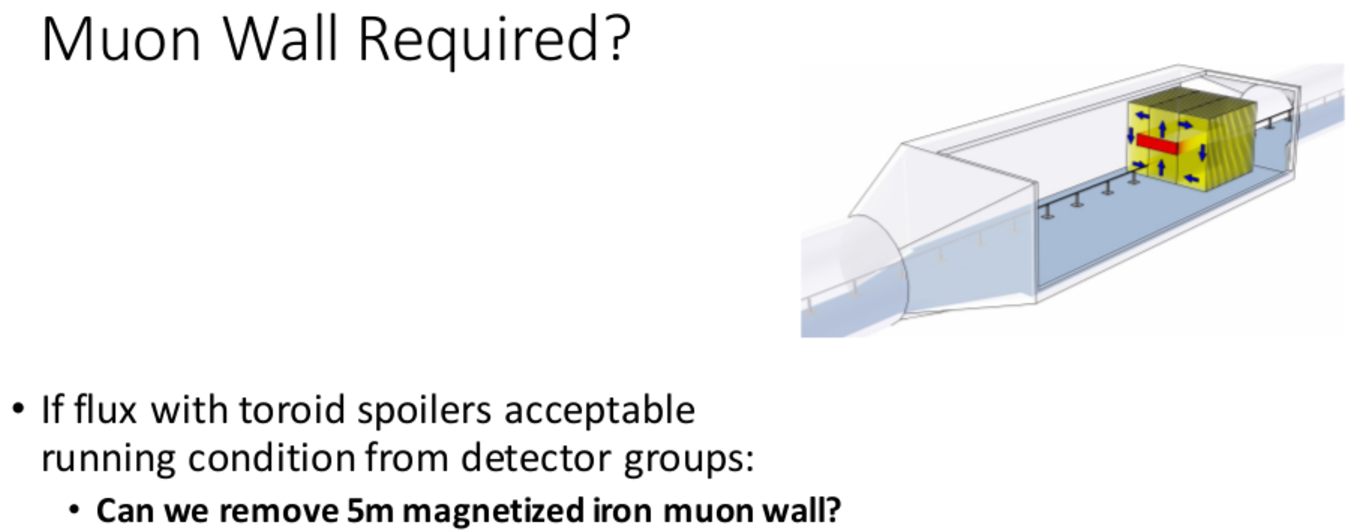
\includegraphics[height=0.5\textheight]{muons_figures/Muon_wall_required.pdf}
\end{center}
\textit{On the other hand:}\\
Removing the wall would mean NO access to IR when the beam is on!\\
And expecting considerably higher rates when going to 1\,TeV $\rightarrow$ maybe wall then neccessary anyway!
\end{frame}

\section{Results}
\subsection{Event displays of muons in the SiD detector}
\begin{frame}{WIRED4 event display - 5 Spoilers + Wall}
\sidlogo
1 train's worth of muons ($\sim$ 515 muons) \textbf{from the positron line only}:
\begin{center}
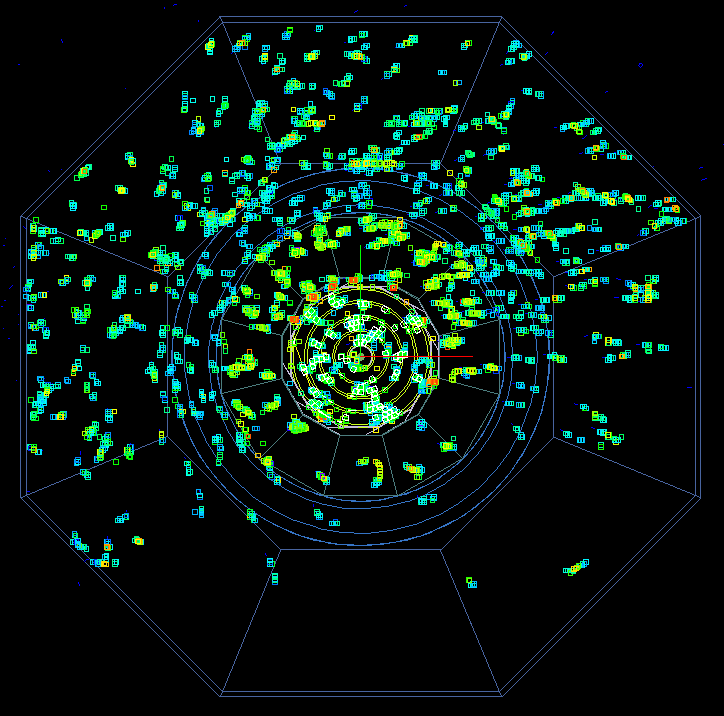
\includegraphics[height=0.6\textheight]{muons_figures/muons_positron_5spoilers_wall_515_xyview_croped.png}
{\tiny xy-view}
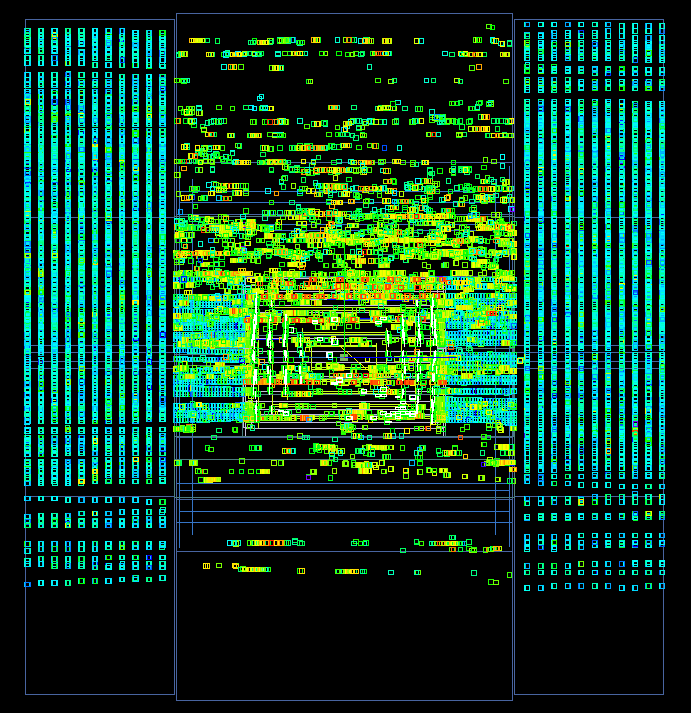
\includegraphics[height=0.6\textheight]{muons_figures/muons_positron_5spoilers_wall_515_zyview_croped.png}
{\tiny zy-view}
\end{center}
Together with the muons from the e\textsuperscript{-} line, there will be \textbf{$\sim$ 900 muons per train in the '5 Spoilers + Wall' scenario}.
\end{frame}
\begin{frame}{WIRED4 event display - 5 Spoilers}
\sidlogo
1 train's worth of muons ($\sim$ 2961 muons) \textbf{from the positron line only}:
\begin{center}
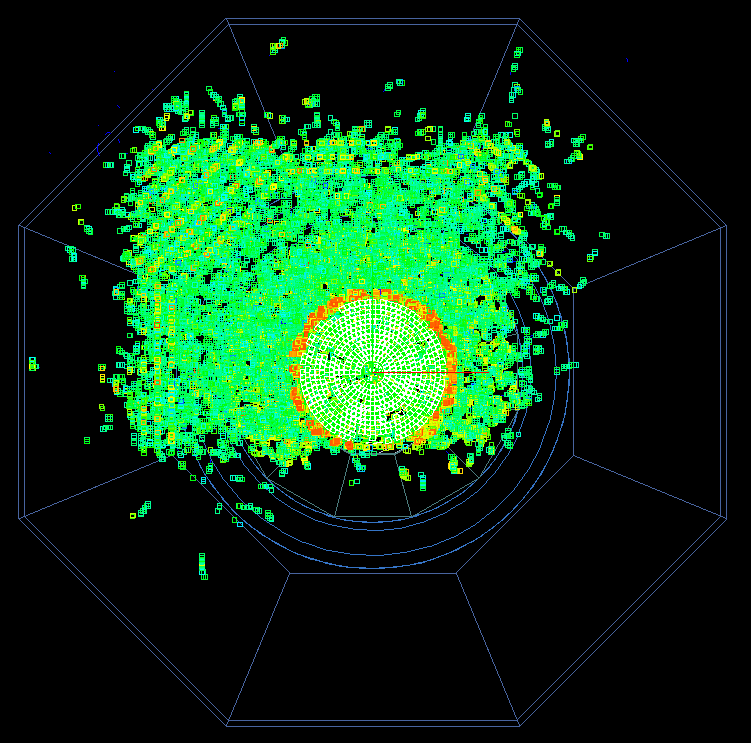
\includegraphics[height=0.6\textheight]{muons_figures/muons_positron_5spoilers_2961_xyview_croped.png}
{\tiny xy-view}
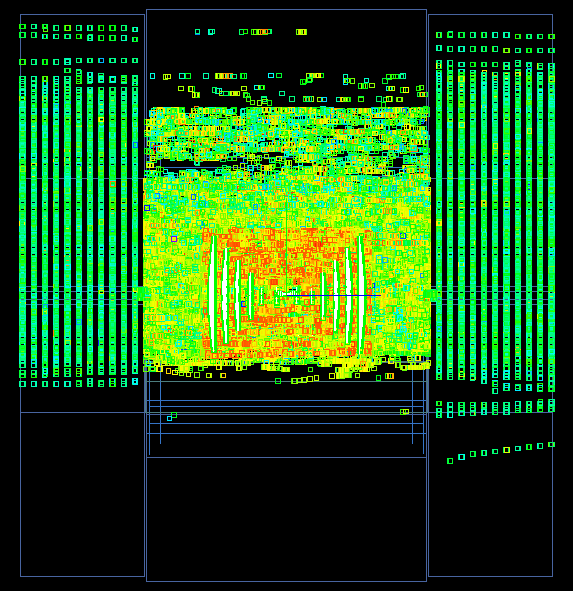
\includegraphics[height=0.6\textheight]{muons_figures/muons_positron_5spoilers_2961_zyview_croped.png}
{\tiny zy-view}
\end{center}
Together with the muons from the e\textsuperscript{-} line, there will be \textbf{$\sim$ 5600 muons per train in the '5 Spoilers' scenario}.\\
The spatial distribution is due to the tunnel shape and its shielding effects.
\end{frame}

%New command: column type
\newcolumntype{P}[1]{>{\centering}p{#1}}

\subsection{Analysis - Total number of hits}
\begin{frame}{Total number of hits}
\sidlogo
\begin{columns}
 \begin{column}{0.23\textwidth}
 \small
  Comparison of the total number of hits in the different SiD subdetectors in the \textcolor{red}{'5 Spoilers'} and the \textcolor{blue}{'5 Spoilers + Wall'} case:
 \end{column}
 \begin{column}{0.8\textwidth}
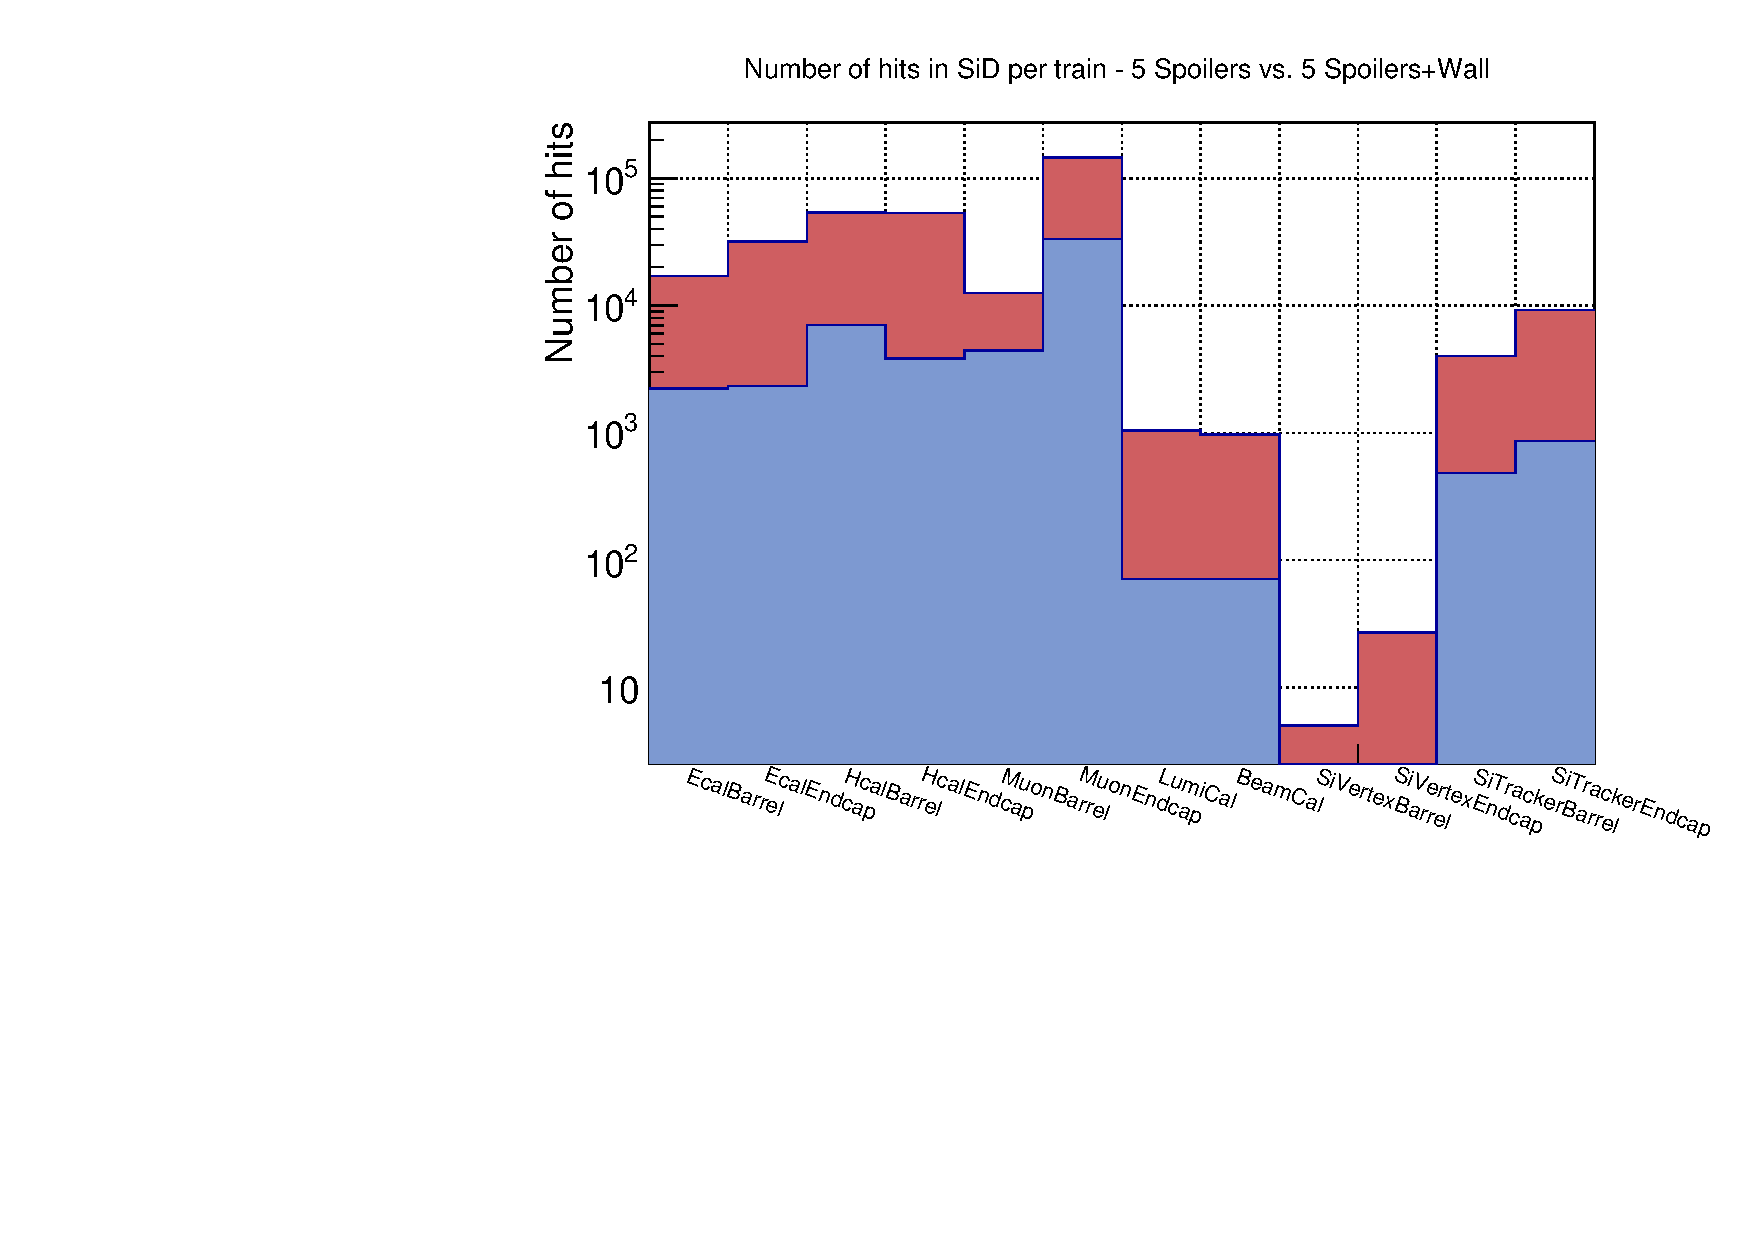
\includegraphics[width=\textwidth]{muons_figures/figures/Hits_in_SiD_subdetectors_MuonSpoilerStudy.pdf}
 \end{column}
\end{columns}
\begin{center}
\begin{tabular}{@{}p{0.343\textwidth}p{0.01\textwidth}p{0.18\textwidth}p{0.01\textwidth}p{0.343\textwidth}p{0.001\textwidth}@{}}
 \centering Vertex detectors & < & \centering ECAL, HCAL & < & \centering MuonEndcaps & \\
  \centering{\scriptsize Smallest effective detector area} & &  \centering{\scriptsize Particle showers} & &  \centering{\scriptsize Biggest effective detector area}&
\end{tabular}
\end{center}
\end{frame}


\subsection{Analysis - Occupancies}
\begin{frame}{Occupancy plots - \small SiTrackerEndcap}
\sidlogo
\begin{columns}
 \begin{column}{0.25\textwidth}
 \small
  Comparison of the muon occupancy in the \textcolor{red}{'5 Spoilers} and the \textcolor{blue}{'5 Spoilers + Wall'} case.\\{\small The \textcolor{green}{buffer depth} of the current sensor design is 4.}\\
  \vspace*{0.2cm}
  {\footnotesize The following occupancy plots are normalized by the first bin.}
 \end{column}
 \begin{column}{0.75\textwidth}
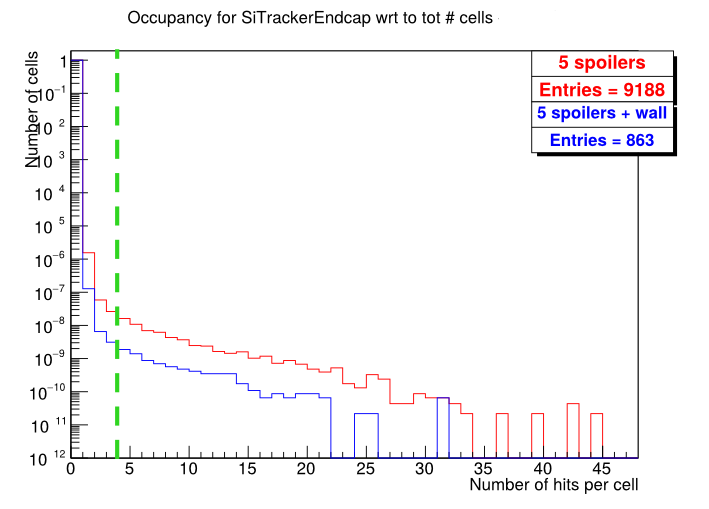
\includegraphics[width=\textwidth]{muons_figures/figures/SiTrackerEndcap_Occupancy.png}
\end{column}
\end{columns}
For both scenarios, 5 Spoilers w/ and w/o Wall, 10$^{-9}$ - 10$^{-7}$ of all cells that get hit have 4 hits.
\end{frame}
\begin{frame}{Occupancy plots - \small EcalEndcap}
\sidlogo
 \begin{center}
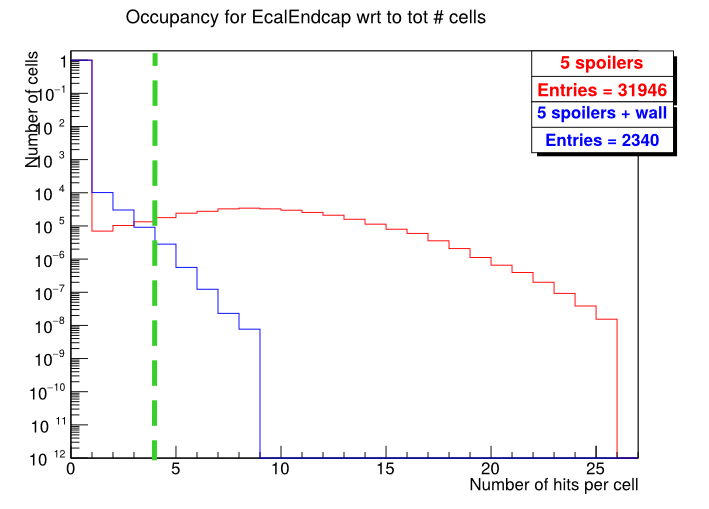
\includegraphics[height=0.62\textheight]{muons_figures/figures/EcalEndcap_Occupancy.png}
\end{center}
\small '5 Spoilers + Wall' seems to do better by an order of magnitude, when looking at a buffer depth of 4. The occupancy is still at a level of only $\sim$10$^{-6}$.\\
\small The '5 Spoiler' case shows up to 27 hits per cell.$\rightarrow$ Constant occupancy for all buffer depths.
\end{frame}

\subsection{Analysis - Dead cells}
\begin{frame}{Dead cells - \small EcalEndcap}
\sidlogo
 \begin{center}
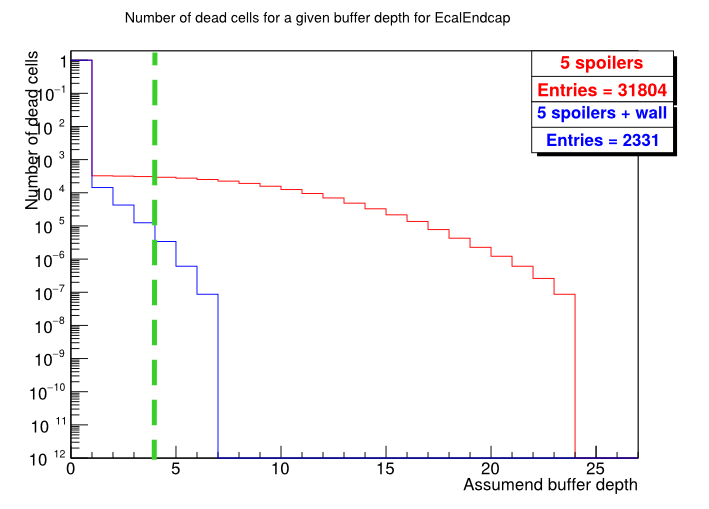
\includegraphics[height=0.65\textheight]{muons_figures/figures/EcalEndcap_DeadCells.png}
\end{center}
\small For an assumed buffer depth of 4, the total number of dead cells is different by about two orders of magnitude. $\rightarrow$ In the '5 Spoiler' case, 10$^{-3}$ cells would have reached the buffer limit.
\end{frame}

\section{Conclusion and Outlook}
\begin{frame}
\textit{Conclusion:}
\begin{itemize}
\item Low energy muons are stopped/deflected by the magnetized wall.
\item High energy muons could be used for tracker alignment.
\item Spatial distributions quite different in the '5 Spoiler' and '5 Spoiler+Wall' scenarios.
\item Number of hits in subdetectors are explained by different geometries.
\item \alert{With the shown evaluation of the muons from the current MUCARLO simulations, SiD would prefer to \textbf{keep the wall}. Additional studies with a comparison to other background sources will be done.}
\end{itemize}
\end{frame}

%--------------------------------------------------------------------------------------------------------------

\section{FLUKA simulation of the ILC Beam Dump}
\begin{frame}
 \centering \LARGE FLUKA simulation of the main beam dump
\end{frame}
\subsection{Project Overview}
{
\usebackgroundtemplate{
\vbox to \paperheight{\vfil
 \tikz\node[opacity=0.1]{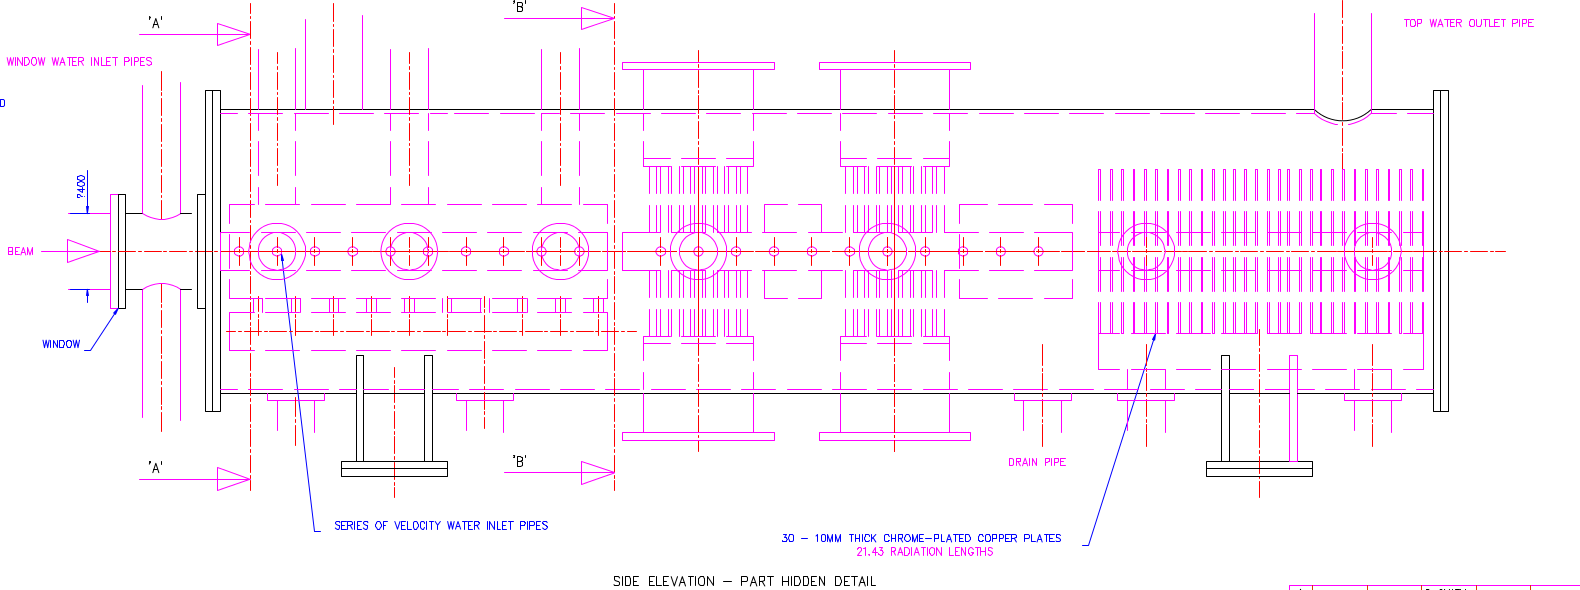
\includegraphics[width=\paperwidth]{BeamDump_figures/TB-0067-300-00-A_yz_view.png}};
 \vfil}
}
\begin{frame}{Neutron Background and Beam Dump Irradiation}
\flukalogo
The 17\,MW\footnote{13.7\,MW average beam power + 20\% margin} beam is dumped into a water tank after collision.\\The activation of the dump surrounding will permit access to the dump area. Neutrons ($\lesssim$\SI{e10}{\per\square\centi\metre\per\year}) are emitted that irradiate the surroundings, and travel back towards the detectors.~\cite{SLAC_FLUKA}\\
\vspace*{0.1cm}
\alert{Goal: Simulating the energy deposition, irradiation, and background particles:}
\begin{enumerate}
 \item Simulating the activation, and the neutrons from the beam dump with FLUKA, using the design drawings by B. Smith~\cite{Smith} to model the dump and the surrounding.
 \item Neutrons through the EXT line: With Benno List (DESY): Python program to plug the real extraction line lattice into FLUKA. Realistic simulation of the interaction between the neutrons and the lattice.
 \item Simulating the neutrons reaching the interaction point in a full detector simulation.
\end{enumerate}
\end{frame}
}

\AtBeginSubsection[] {
  \begin{frame}<beamer>
     \tableofcontents[currentsection,
     currentsubsection,
     %hideothersubsections,
     subsectionstyle=show/shaded/hide,
     subsubsectionstyle=show/show/hide]
  \end{frame}
}

\subsection{The Beam Dump Designs}
\begin{frame}{\textbf{Shielding walls}: 0-TB-0067-404-00-A}
\begin{center}
\only<1>{
Design drawings by B. Smith, 2006-2007~\cite{Smith}
\includegraphics[width=0.83\textwidth]{BeamDump_figures/0067_404-Shielding.png}
 }
 \only<2>{
  \includegraphics[width=0.65\textwidth,angle=90]{BeamDump_figures/0067_404-Shielding_zoom.png}
  }
\end{center}
\end{frame}

\begin{frame}{\textbf{Design 1}: 0-TB-0067-210-00-A}
\begin{center}
  \includegraphics[width=0.92\textwidth]{BeamDump_figures/TB-0067-210-00-A.png}
\end{center}
\end{frame}
{
\usebackgroundtemplate{
\vbox to \paperheight{\vspace*{1.2cm}
 \tikz\node[opacity=0.3]{\hspace*{0.6cm} \includegraphics[width=0.92\textwidth]{BeamDump_figures/TB-0067-210-00-A.png}};
 \vfil}}
\begin{frame}{\textbf{Design 1}: 0-TB-0067-210-00-A}
\begin{columns}
 \begin{column}{0.5\textwidth}
  Vessel:
  \begin{itemize}
   \item Diameter: 1.5\,m
   \item Length: 6.5\,m
   \item 316L Stainless Steel
   \item Water pressure: 10\,bar
  \end{itemize}
  Window:
  \begin{itemize}
   \item Diameter: 300\,mm
   \item Thickness: 1\,mm
   \item Titanium alloy: Ti-6Al-4V 
  \end{itemize}
 \end{column}
 \begin{column}{0.5\textwidth}
  27\,X\textsubscript{0} needed to stop a 500\,GeV beam:
  \begin{itemize}
   \item Water: 18\,X\textsubscript{0}
   \item Water cooled copper plates: 9\,X\textsubscript{0} = 126\,mm
  \end{itemize}  
 \end{column}
\end{columns}

\end{frame}
}

\begin{frame}{\textbf{Design 2}: 0-TB-0067-300-00-A}
\begin{center}
  \includegraphics[width=0.92\textwidth]{BeamDump_figures/TB-0067-300-00-A.png}
 \end{center}
\end{frame}
{
\usebackgroundtemplate{
\vbox to \paperheight{\vspace*{1.2cm}
 \tikz\node[opacity=0.3]{\hspace*{0.6cm} \includegraphics[width=0.92\textwidth]{BeamDump_figures/TB-0067-300-00-A.png}};
 \vfil}}
\begin{frame}{\textbf{Design 2}: 0-TB-0067-210-00-A}
\begin{columns}
 \begin{column}{0.5\textwidth}
  Vessel:
  \begin{itemize}
   \item Diameter: 1.5\,m
   \item Length: 6.5\,m
   \item 316L Stainless Steel
   \item Water pressure: 10\,bar
  \end{itemize}
  Window:
  \begin{itemize}
   \item Diameter: 300\,mm
   \item Thickness: 1\,mm
   \item Titanium alloy: Ti-6Al-4V 
  \end{itemize}
 \end{column}
 \begin{column}{0.5\textwidth}
  27\,X\textsubscript{0} needed to stop a 500\,GeV beam:
  \begin{itemize}
   \item Water: 18\,X\textsubscript{0}
   \item Water cooled copper plates: 9\,X\textsubscript{0} = 126\,mm
  \end{itemize}  
    Additionally high water pressure section:
  \begin{itemize}
   \item Titanium tubes, 4\,cm diameter
   \item High pressure water flow
   \item In total 1.98\,X\textsubscript{0}
  \end{itemize} 
 \end{column}
\end{columns}

\end{frame}
}

\subsection{The FLUKA simulation}
\begin{frame}
For the simulation, the ILC1000B was chosen as the scenario with the largest beam power.\\
\vspace*{0.5cm}
 ILC1000B:
 \begin{itemize}
  \item Beam energy: 500\,GeV
  \item Bunch population: 1.74e10
  \item Bunch size: \textsigma\textsubscript{x} = 2.4\,mm, \textsigma\textsubscript{y} = 0.22\,mm
  \item Bunches per train: 2450
  \item Bunch train duration: 896.7\,\textmu s
 \end{itemize}
\vspace*{0.2cm}
Beams are considered un-collided and un-disrupted.
\end{frame}


\subsubsection{Deposited Energy and Dose}
\begin{frame}{Deposited Energy per bunch}
\begin{center}
\hspace*{1.6cm} Design 1 \hfill Design 2 \hspace*{1.8cm} \\
  \includegraphics[width=0.52\textwidth]{BeamDump_figures/Energy_deposition_xz_Design1.pdf}
    \includegraphics[width=0.52\textwidth]{BeamDump_figures/Energy_deposition_xz_Design2.pdf}
\end{center}
 Shielding walls seem to stop particles fluxes well, but large scattering in Design 2 at high water pressure sections leads to energy deposition outside the walls.
\end{frame}
\begin{frame}{Maximum Deposited Energy over Z per bunch}
\begin{center}
\hspace*{1.6cm} Design 1 \hfill Design 2 \hspace*{1.8cm} \\
  \includegraphics[width=0.51\textwidth]{BeamDump_figures/Energy_deposition_1DMax_z_Design1_withLabels.pdf}
    \includegraphics[width=0.51\textwidth]{BeamDump_figures/Energy_deposition_1DMax_z_Design2_withLabels.pdf}
\end{center}
  \textbf{Maximum deposited energy} within the water tank up to \textbf{10\textsuperscript{8}-10\textsuperscript{9}\,GeV/cm\textsuperscript{3} (= 0.016 - 0.16 J/cm\textsuperscript{3}) per bunch}.
\end{frame}


\begin{frame}{Instantaneous Dose Equivalent per bunch}
\begin{center}
\hspace*{1.8cm} Design 1 \hfill Design 2 \hspace*{1.8cm} \\
  \includegraphics[width=0.52\textwidth]{BeamDump_figures/Dose_equivalent_total_Design1.pdf}
    \includegraphics[width=0.52\textwidth]{BeamDump_figures/Dose_equivalent_total_Design2.pdf}
\end{center}
The two designs show comparable distributions of the dose equivalent.
\end{frame}
\begin{frame}{Maximum Instantaneous Dose Equivalent over Z}
\begin{center}
\hspace*{2cm} Design 1 \hfill Design 2 \hspace*{1.8cm} \\
  \includegraphics[width=0.51\textwidth]{BeamDump_figures/Dose_equivalent_1DMax_z_Design1_withLabels.pdf}
    \includegraphics[width=0.51\textwidth]{BeamDump_figures/Dose_equivalent_1DMax_z_Design2_withLabels.pdf}
\end{center}
\textbf{Maximum dose equivalent} within the water tank up to \textbf{100\,Sv per bunch}. Peaks in distributions at locations with lots of material.
\end{frame}
\begin{frame}
\textbf{After one month of beam operation}, the beam is turned off.\\
Different \textbf{cooling times} are considered:\\
\textbf{1 minute, 1 hour, 1 day, 1 month, and 1 year}\\
  \frametitle{Dose equivalent after cooling times - \textbf{Design 1}}
  \hypertarget{coolingtimesprev_Design1}{}
  \begin{center}
    \hspace*{1cm} Instantaneous \hfill After 1 minute \hfill After 1 hour \hspace*{1.2cm} \\
  \hyperlink{Dose_equivalent_Design1}{\includegraphics[width=0.3\textwidth]{BeamDump_figures/Dose_equivalent_total_Design1.pdf}}
  \hyperlink{Dose_equivalent_minute_Design1}{\includegraphics[width=0.3\textwidth]{DoseEQ_Time/Design1_1.pdf}}
  \hyperlink{Dose_equivalent_hour_Design1}{\includegraphics[width=0.3\textwidth]{DoseEQ_Time/Design1_2.pdf}}\\
    \hspace*{1.2cm} After 1 day \hfill After 1 month \hfill After 1 year\hspace*{1.4cm} \\
  \hyperlink{Dose_equivalent_day_Design1}{\includegraphics[width=0.3\textwidth]{DoseEQ_Time/Design1_3.pdf}}
  \hyperlink{Dose_equivalent_month_Design1}{\includegraphics[width=0.3\textwidth]{DoseEQ_Time/Design1_4.pdf}}
  \hyperlink{Dose_equivalent_year_Design1}{\includegraphics[width=0.3\textwidth]{DoseEQ_Time/Design1_5.pdf}}
 \end{center}
\end{frame}
\begin{frame}
  \frametitle{Dose equivalent after cooling times - \textbf{Design 2}}
  \hypertarget{coolingtimesprev_Design2}{}
  \begin{center}
    \hspace*{1cm} Instantaneous \hfill After 1 minute \hfill After 1 hour \hspace*{1.2cm} \\
  \hyperlink{Dose_equivalent_Design2}{\includegraphics[width=0.3\textwidth]{BeamDump_figures/Dose_equivalent_total_Design2.pdf}}
  \hyperlink{Dose_equivalent_minute_Design2}{\includegraphics[width=0.3\textwidth]{DoseEQ_Time/Design2_1.pdf}}
  \hyperlink{Dose_equivalent_hour_Design2}{\includegraphics[width=0.3\textwidth]{DoseEQ_Time/Design2_2.pdf}}\\
    \hspace*{1.2cm} After 1 day \hfill After 1 month \hfill After 1 year\hspace*{1.4cm} \\
  \hyperlink{Dose_equivalent_day_Design2}{\includegraphics[width=0.3\textwidth]{DoseEQ_Time/Design2_3.pdf}}
  \hyperlink{Dose_equivalent_month_Design2}{\includegraphics[width=0.3\textwidth]{DoseEQ_Time/Design2_4.pdf}}
  \hyperlink{Dose_equivalent_year_Design2}{\includegraphics[width=0.3\textwidth]{DoseEQ_Time/Design2_5.pdf}}
 \end{center}
\end{frame}
\begin{frame}{Dose Rate over Time}
The dose rate measured at the longitudinal shower maximum inside the vessel over time:
\begin{center}
  \includegraphics[width=0.7\textwidth]{BeamDump_figures/DoseEQ_Time_Comparison.pdf}
\end{center}
\textbf{After one year}, the dose rate drops to \\\textbf{$\sim$ 0.1\,mSv/s} for \textcolor{Red}{Design 1} and to \textbf{$\sim$ 10\,mSv/s} for \textcolor{Blue}{Design 2}.
\end{frame}

\AtBeginSubsubsection[] {
  \begin{frame}<beamer>
     \tableofcontents[currentsection,
     currentsubsection,
     %hideothersubsections,
     subsectionstyle=show/shaded/hide,
     subsubsectionstyle=show/show/hide]
  \end{frame}
}



\subsubsection{Particle Fluxes}

\begin{frame}{Neutron fluxes from one bunch: \textbf{Design 1}}
\begin{columns}
 \begin{column}{0.5\textwidth}
    \includegraphics[width=\textwidth]{BeamDump_figures/Neutron_flux_xz_Design1.pdf}
 \end{column}
 \begin{column}{0.5\textwidth}
  The neutrons spread more in the positive x and y-direction. Within the tank, the neutrons are mainly produced in the water vortex system. When the beam is stopped by the copper plates, the neutron production rate decreases.
 \end{column}
\end{columns}
\hspace*{1cm} x-direction \hfill y-direction \hfill z-direction \hspace*{1cm} \\
  \includegraphics[width=0.31\textwidth]{BeamDump_figures/Neutron_flux_1DMax_x_Design1.pdf}\hfill
  \includegraphics[width=0.31\textwidth]{BeamDump_figures/Neutron_flux_1DMax_y_Design1.pdf}\hfill
  \includegraphics[width=0.31\textwidth]{BeamDump_figures/Neutron_flux_1DMax_z_Design1_withLabels.pdf}
\end{frame}
\begin{frame}{Neutron fluxes from one bunch: \textbf{Design 2}}
\begin{columns}
 \begin{column}{0.5\textwidth}
    \includegraphics[width=\textwidth]{BeamDump_figures/Neutron_flux_xz_Design2.pdf}
 \end{column}
 \begin{column}{0.5\textwidth}
  The neutrons again spread more in the positive x and y-direction. Within the tank, the point of highest neutron production is the high pressure water system. The production rate again decreases with the beam being stopped by the copper plates.
 \end{column}
\end{columns}
\hspace*{1cm} x-direction \hfill y-direction \hfill z-direction \hspace*{1cm} \\
  \includegraphics[width=0.31\textwidth]{BeamDump_figures/Neutron_flux_1DMax_x_Design2.pdf}\hfill
  \includegraphics[width=0.31\textwidth]{BeamDump_figures/Neutron_flux_1DMax_y_Design2.pdf}\hfill
  \includegraphics[width=0.31\textwidth]{BeamDump_figures/Neutron_flux_1DMax_z_Design2_withLabels.pdf}
\end{frame}


\section{Summary and Outlook}
\begin{frame}{Conclusion}
 \flukalogo
 Water beam dump designs:
 \begin{itemize}
  \item The simulations of the two water beam dump designs by B. Smith show \textbf{comparable results}.
  \item The dose rate of the beam dump surrounding is still after one year in the order of \textbf{10\textsuperscript{-1}\,mSv/s}.
  \item \textbf{Design 2} seems to be \textbf{more elaborated regarding the water cooling flow system}.
  This leads to \textbf{larger spreads in the energy deposition} due to the high water pressure sections.
 \end{itemize}
 \visible<2->{
 \vspace*{0.2cm}
 FOR FUN:
 \begin{itemize}
  \item Simulated simplified gas dump filled with Nitrogen
  \item Adopting ideas from dump design studies for TESLA done at DESY.
  \item Copper walls with a thickness of $\sim$\,60\,cm
 \end{itemize}
 \begin{center}
  \includegraphics[width=0.5\textwidth]{Gas_dump/Geometry.png}
 \end{center}
  }
\end{frame}
\begin{frame}{For Fun: Nitrogen Gas Dump}
 \flukalogo
 \includegraphics[width=0.45\textwidth]{Gas_dump/Energy_Deposition.pdf}\hfill
 \includegraphics[width=0.45\textwidth]{Gas_dump/Dose_equivalent.pdf}\\
 \includegraphics[width=0.45\textwidth]{Gas_dump/Dose_equivalent_1day.pdf}\hfill
 \includegraphics[width=0.45\textwidth]{Gas_dump/Dose_equivalent_1month.pdf}
\end{frame}

\begin{frame}{Summary and outlook}
 \flukalogo
 Goals for the next months:
\begin{itemize}
 \item Studying the influence of the water composition (amount of deuterium),
 \item the influence of the composition of the steel vessel and the concrete shielding,
 \item simulating the neutron flux through the EXT line,
 \item the number of neutrons reaching the IP,
 \item the neutron occupancy in SiD.
\end{itemize}
\end{frame}

%--------------------------------------------------------------------------------------------------------------

\section{Pair background studies for the new ILC250 schemes}
\begin{frame}
 \centering \LARGE Pair background studies for the new ILC250 schemes
\end{frame}

\begin{frame}{ILC250 Beam Parameter Sets}
 \begin{table}
\caption{Possible beam parameter sets for the ILC250 stage. The table only lists the parameters that are to be changed with respect to the original ILC250 parameters given in the Technical Design Report (TDR)~\cite[p. 11]{TDR1}.}
\label{tab:Parameters}
\centering
\begin{tabularx}{0.55\textwidth}{llll}
\hline\hline
\textbf{Set}  & \textbf{$\epsilon_x$ [\murm m]} & \textbf{$\beta_x$ [mm]} & \textbf{$\beta_y$ [mm]}\\
\hline
\cline{1-4}
\hline
 TDR & 10 & 13.0 & 0.41\\
 (A) & 5 & 13.0 & 0.41\\
 (B) & 5 & 9.19 & 0.41\\
 (C) & 5 & 9.19 & 0.58\\
\hline\hline
\end{tabularx}
\end{table}
Reduced emittance leads to stronger beam-beam interactions, and therefore to increased \positron \electron pair background.
\end{frame}

\subsection{Pair background envelopes}
\begin{frame}{Pair background envelopes}
 \begin{figure}
\centering
\begin{subfigure}[t]{0.35\textwidth}
\centering
\includegraphics[width=\textwidth]{ILC250_figures/Helix_tracks_xz_100bunches_250GeV_5T_DanielJeans-1.jpg}
\caption{ILC250 set (TDR)}
\end{subfigure}
\hspace*{0.1cm}
\begin{subfigure}[t]{0.35\textwidth}
\centering
\includegraphics[width=\textwidth]{ILC250_figures/Helix_tracks_xz_80bunches_250GeV_5T_Reduced_Emittance_x-1.jpg}
\caption{ILC250 set (A)}
\end{subfigure}
\\
\begin{subfigure}[t]{0.35\textwidth}
\centering
\includegraphics[width=\textwidth]{ILC250_figures/Helix_tracks_xz_50bunches_250GeV_5T_Reduced_Emittance_x_Reduced_Beta_x-1.jpg}
\caption{ILC250 set (B)}
\end{subfigure}
\hspace*{0.1cm}
\begin{subfigure}[t]{0.35\textwidth}
\centering
\includegraphics[width=\textwidth]{ILC250_figures/Helix_tracks_xz_50bunches_250GeV_5T_Reduced_Emittance_x_Reduced_Beta_x_Increased_Beta_y-1.jpg}
\caption{ILC250 set (C)}
\end{subfigure}
\caption{Pair background density for the different ILC250 beam parameter sets.
The beam pipe is represented by the red solid lines.}
\label{fig:Envelopes}
\end{figure}

\end{frame}

\begin{frame}{Projection of the pair background density along x}
\begin{center}
 \includegraphics[width=0.72\textwidth]{ILC250_figures/HelixEnvelope_Projection_Comparison_250GeV_parametersets_NEWSETNAMES.png}
\end{center}
The envelopes are in all schemes well contained within in the beam pipe. Less than 10 particles per bunch crossing are to be expected outside the beam pipe.
\end{frame}

\begin{frame}{SiD Vertex Detector Occupancy: All layers}
 \begin{figure}
\centering
\begin{subfigure}[t]{0.45\textwidth}
\centering
\includegraphics[width=\textwidth]{ILC250_figures/Occupancy_Comparison_All_layers_wrt__cells_ILC250_ALL_SETS_6Sep2017_NEWSETNAMES.png}
\caption{Normalized Occumancy: Number of cells containing a certain amount of hits, normalized by the total number of cells of the vertex detector.}
\end{subfigure}
\hspace*{0.1cm}
\begin{subfigure}[t]{0.45\textwidth}
\centering
\includegraphics[width=\textwidth]{ILC250_figures/Occupancy_Comparison_All_layers_deadcells_ILC250_ALL_SETS_6Sep2017_NEWSETNAMES.png}
\caption{Ratio of dead cells in comparison to all cells of the vertex detector.}
\end{subfigure}
\end{figure}
\end{frame}

\begin{frame}{SiD Vertex Detector Occupancy: Layer 0}
\begin{center}
 \includegraphics[width=0.6\textwidth]{ILC250_figures/Occupancy_Comparison_Layer_0_numcells_ILC250_ALL_SETS_6Sep2017_NEWSETNAMES.png}
\end{center}
The occupancy in layer 0 for the new sets is significantly increased with respect to the TDR scheme.\\
SiD is confident that the occupancy can be accommodated in the design of the pixel detector.\\
Studies with smaller original L* of \SI{3.5}{\meter} are ongoing. $\rightarrow$ \alert{Stay tuned!}
\end{frame}


%---------------------------------------------------------------------------------

\section*{The end}
{
\usebackgroundtemplate{
 \tikz\node[opacity=0.1]{\includegraphics[width=\paperwidth,resolution=200]{figures/ilc-Comic.png}};
 % \tikz\node[opacity=0.2]{\centering\includegraphics[height=\paperheight]{figures/Iwatecomics.jpg}};
 }
\begin{frame}
\ilclogo
\begin{center}
\textcolor{RubineRed}{
	\LARGE Thanks!\\
}
\end{center}
\end{frame}
}

\section*{References}
\begin{thebibliography}{9}
\begin{frame}{References}
\setbeamertemplate{bibliography item}[text]
\bibitem{Smith} B. Smith (Rutherford Lab), \emph{Design drawings 0-TB-0067-300-00-A, 0-TB-0067-210-00-A, 0-TB-0067-404-00-A}, Dec. 2006 - Jan. 2007
\bibitem{Smith_Report} B. Smith (CCLRC Technology Department), \emph{18\,MW Water Beam Dump Concept}, Report 088-D-006-01, Jan. 2007
\bibitem{SLAC_FLUKA} S. Darbha, \emph{Simulation of Neutron Backgrounds from the ILC Extraction Line Beam Dump}, SLAC-TN-07-013, Aug. 2007
\bibitem{NIM_paper} P. Satyamurthy, et al., \emph{Design of an 18\,MW vortex flow water beam dump for 500\,GeV electrons/positrons of an international linear collider}, NIM A 679 (2012) 67-81
\bibitem{CLIC_dump} A. Mereghetti, et al., \emph{FLUKA and Thermo-Mechanical Studies for the CLIC Main Dump}, CLIC-Note-876, Mach 2011
\end{frame}
\begin{frame}{References}
\bibitem{Concrete} K. Okuno, et al., \emph{Application of neutron shield concrete to neutron scattering instrument TAIKAN in J-PARC}, Progress in Nuclear Science and Technology, Vol. 4, pp 619-622, 2014
\end{frame}
\begin{frame}{References}
\bibitem{TDR1} T. Behnke, et al., \emph{The International Linear Collider - Technical Design Report, Volume 1}, 2013.
\end{frame}
\end{thebibliography}

%--------------------------------------------------------------------------------
\appendix

\begin{frame}
\begin{center}
\LARGE Additional Material
\end{center}
  \tableofcontents
\end{frame}

\section{ILC}

\subsection{The ILC beam parameters}
\begin{frame}{ILC baseline parameters}
\ilclogo
\begin{center}
	\includegraphics[width=\textwidth]{figures/ILCTDR-VOLUME_3-PART_II_ILCparameters.pdf}
\end{center}
\end{frame}
\begin{frame}{ILC parameters for the different upgrade stages}
\ilclogo
\begin{center}
	\includegraphics[width=0.8\textwidth]{figures/ILCTDR-VOLUME_3-PART_II_ILCparametersUpgrades.pdf}
\end{center}
\end{frame}

\section{BDS muons}
\subsection{Analysis - Spatial distributions}
\begin{frame}{Explanation of spatial distributions}
\sidlogo
 \begin{center}
\includegraphics[height=0.85\textheight]{muons_figures/Explanation_Spatial_distribution_NEW.pdf}
\end{center}
\end{frame}

\subsection{Analysis - Energy distributions}
\begin{frame}{Energy distribution of muons}
\sidlogo
\begin{columns}
 \begin{column}{0.25\textwidth}
 \small
  Comparison of the muon energies in the \textcolor{red}{'5 Spoilers'} and the \textcolor{blue}{'5 Spoilers + Wall'} case:
 \end{column}
 \begin{column}{0.75\textwidth}
  \includegraphics[width=\textwidth]{muons_figures/figures/muon_energy.pdf}
 \end{column}
\end{columns}
In the 'Spoiler + Wall' case, the lower energy muons are either stopped or deflected by the magnetized wall.
\end{frame}

\subsection{Analysis - SiD hit distribution}
\begin{frame}{Explanation of hit number distribution -\\ \small Spatial distribution in the MuonEndcaps}
\sidlogo
 \begin{center}
\includegraphics[height=0.78\textheight]{muons_figures/Explanation_Hits_Subdetectors.pdf}
\end{center}
\end{frame}

\subsection{Analysis - Dead cells}
\begin{frame}{Dead cells - \small SiTrackerEndcap}
\sidlogo
 \begin{center}
\includegraphics[height=0.65\textheight]{muons_figures/figures/SiTrackerEndcap_DeadCells.png}
\end{center}
\small For an assumed buffer depth of 4, the total number of dead cells is different by an order of magnitude. $\rightarrow$ In the '5 Spoiler' case, 10$^{-7}$ cells would have reached the buffer limit.
\end{frame}

\subsection{Analysis - Time distributions}
\begin{frame}{Creation time distribution}
\sidlogo
All of the primary muons are created up to 0.5\,ns after the bunch passing the material.
 \begin{center}
\includegraphics[height=0.65\textheight]{muons_figures/figures/muon_creationtime.pdf}
\end{center}
The lower energy muons, which have a broader creation time, do not reach the detector in the '5 Spoilers + Wall' case.
\end{frame}
\begin{frame}{Hit Time distribution - \small MuonEndcaps}
\sidlogo
 \begin{center}
\includegraphics[height=0.65\textheight]{muons_figures/figures/muon_hittime_all_layers_MuonEndcap.pdf}
\end{center}
Muons are first hitting the MuonEndcaps as the most outer subdetector.
\end{frame}
\begin{frame}{Hit Time distribution - \small EcalEndcaps}
\sidlogo
Hit time distributions for \\
\hspace*{0.6cm} the PRIMARY MUONS and the SHOWER PARTICLES:
 \begin{center}
\includegraphics[height=0.5\textheight]{muons_figures/figures/muon_hittime_all_layers_EcalEndcap.pdf}
\includegraphics[height=0.5\textheight]{muons_figures/figures/muon_hittime_all_layers_shower_EcalEndcap.pdf}
\end{center}
The primary muons leave hits between 12 and $\sim$ 50\,ns after the bunch crossing, whereas the shower particles hit the EcalEndcaps about 60\,ns after the crossing.
\end{frame}
\begin{frame}{Hit Time distribution - \small SiTrackerEndcaps}
\sidlogo
Hit time distributions for \\
\hspace*{0.6cm} the PRIMARY MUONS and the SHOWER PARTICLES:
 \begin{center}
\includegraphics[height=0.5\textheight]{muons_figures/figures/muon_hittime_all_layers_SiTrackerEndcap.pdf}
\includegraphics[height=0.5\textheight]{muons_figures/figures/muon_hittime_all_layers_shower_SiTrackerEndcap.pdf}
\end{center}
The primary muons leave hits between 12 and $\sim$ 40\,ns after the bunch crossing, whereas the shower particles hit the Tracker endcaps about 40-100\,ns after the crossing.
\end{frame}

\section{FLUKA simulation}

\subsection{Deposited Energy}
\begin{frame}{Total Deposited Energy per region per bunch}
\begin{center}
\begin{tabular}{|c|c|c|c|}
\hline
 Dep. Energy [J] & \textbf{Water} & \textbf{Vessel} & \textbf{Window} \\
\hline
Design 1 & 233.24 & 5.14 & 0.0019\\
\hline
\hline
Design 2 & 240.67 & 4.36 & 0.0018\\
\hline
\end{tabular}
\end{center}
\begin{center}
\begin{tabular}{|c|c|c|c|}
\hline
 Dep. Energy [J] & \textbf{Cu plate 1} & \textbf{Last Cu plate} & \textbf{Iron shielding} \\
\hline
Design 1 & 4.44 & 1.46 & 5.09\\
\hline
\hline
Design 2 & 1.58 & 0.13 & 5.87\\
\hline
\end{tabular}
\end{center}

Numbers comparable to former FLUKA simulations of beam dump concepts for the ILC~\cite{NIM_paper} and CLIC~\cite{CLIC_dump}.
\end{frame}

\subsection{Residual nuclei}
\begin{frame}{Residual nuclei after cooling times}
\textbf{After one month of beam operation}, the beam is turned off.\\
Different \textbf{cooling times} are considered:\\
\textbf{1 minute, 1 hour, 1 day, 1 month, and 1 year}\\
\vspace*{0.3cm}
\hspace*{1.8cm} Design 1 \hfill Design 2 \hspace*{2.3cm} \\
  \begin{center}
  \animategraphics[controls,loop,width=0.49\textwidth]{0.5}{Residual_Time/Design1_}{1}{5}
  \animategraphics[controls,loop,width=0.49\textwidth]{0.5}{Residual_Time/Design2_}{1}{5}
  \end{center}
\end{frame}
\begin{frame}
  \frametitle{Residual nuclei after cooling times - \textbf{Design 1}}
  \hypertarget{residualtimesprev_Design1}{}
  \begin{center}
    \hspace*{1cm} Instantaneous \hfill After 1 minute \hfill After 1 hour \hspace*{1.2cm} \\
  \hyperlink{Residual_nuclei_Design1}{\includegraphics[width=0.3\textwidth]{BeamDump_figures/Residual_nuclei_Design1.pdf}}
  \hyperlink{Residual_nuclei_minute_Design1}{\includegraphics[width=0.3\textwidth]{Residual_Time/Design1_1.pdf}}
  \hyperlink{Residual_nuclei_hour_Design1}{\includegraphics[width=0.3\textwidth]{Residual_Time/Design1_2.pdf}}\\
    \hspace*{1cm} After 1 day \hfill After 1 month \hfill After 1 year\hspace*{1.4cm} \\
  \hyperlink{Residual_nuclei_day_Design1}{\includegraphics[width=0.3\textwidth]{Residual_Time/Design1_3.pdf}}
  \hyperlink{Residual_nuclei_month_Design1}{\includegraphics[width=0.3\textwidth]{Residual_Time/Design1_4.pdf}}
  \hyperlink{Residual_nuclei_year_Design1}{\includegraphics[width=0.3\textwidth]{Residual_Time/Design1_5.pdf}}
 \end{center}
\end{frame}
\begin{frame}
  \frametitle{Residual nuclei after cooling times - Design 2}
  \hypertarget{residualtimesprev_Design2}{}
  \begin{center}
    \hspace*{1cm} Instantaneous \hfill After 1 minute \hfill After 1 hour \hspace*{1.2cm} \\
  \hyperlink{Residual_nuclei_Design2}{\includegraphics[width=0.3\textwidth]{BeamDump_figures/Residual_nuclei_Design2.pdf}}
  \hyperlink{Residual_nuclei_minute_Design2}{\includegraphics[width=0.3\textwidth]{Residual_Time/Design2_1.pdf}}
  \hyperlink{Residual_nuclei_hour_Design2}{\includegraphics[width=0.3\textwidth]{Residual_Time/Design2_2.pdf}}\\
    \hspace*{1cm} After 1 day \hfill After 1 month \hfill After 1 year\hspace*{1.4cm} \\
  \hyperlink{Residual_nuclei_day_Design2}{\includegraphics[width=0.3\textwidth]{Residual_Time/Design2_3.pdf}}
  \hyperlink{Residual_nuclei_month_Design2}{\includegraphics[width=0.3\textwidth]{Residual_Time/Design2_4.pdf}}
  \hyperlink{Residual_nuclei_year_Design2}{\includegraphics[width=0.3\textwidth]{Residual_Time/Design2_5.pdf}}
 \end{center}
\end{frame}

\begin{frame}{Number of radio-nuclides}
The presence of certain nuclei is dependent on the choice of materials used for the dump vessel, the shielding\footnote{Composition of concrete and neutron shielding concrete was taken from \cite{Concrete}.} etc.
\begin{center}
\hspace*{1cm} Tritium flux: Design 1 \hfill Tritium flux: Design 2 \hspace*{1cm} \\
  \includegraphics[width=0.52\textwidth]{BeamDump_figures/Tritium_flux_xz_Design1.pdf}
    \includegraphics[width=0.52\textwidth]{BeamDump_figures/Tritium_flux_xz_Design2.pdf}
 \end{center}
\end{frame}

\subsection{Particle Fluxes}
\begin{frame}{Electron and Photon fluxes from one bunch}
\begin{center}
Design 1 \hspace*{1.4cm} Electrons \hfill Photons \hspace*{3.1cm} \\
 \includegraphics[width=0.37\textwidth]{BeamDump_figures/Electron_flux_xz_Design1.pdf}
  \includegraphics[width=0.37\textwidth]{BeamDump_figures/Photon_flux_xz_Design1.pdf}\\
Design 2 \hspace*{1.4cm} Electrons \hfill Photons \hspace*{3.1cm} \\ 
\includegraphics[width=0.37\textwidth]{BeamDump_figures/Electron_flux_xz_Design2.pdf}
  \includegraphics[width=0.37\textwidth]{BeamDump_figures/Photon_flux_xz_Design2.pdf}
\end{center}
\end{frame}
\begin{frame}{Proton fluxes}
\begin{center}
\hspace*{2cm} Design 1 \hfill Design 2 \hspace*{2cm} \\
  \includegraphics[width=0.52\textwidth]{BeamDump_figures/Proton_flux_xz_Design1.pdf}
    \includegraphics[width=0.52\textwidth]{BeamDump_figures/Proton_flux_xz_Design2.pdf}
\end{center}
\end{frame}


\section{Zoom Plots}
\begin{frame}
  \begin{center}
    \huge
    ZOOM PLOTS\\
    \tiny
    Here be dragons
  \end{center}
\end{frame}
\begin{frame}[plain]
 \hypertarget{Dose_equivalent_Design1}{\hyperlink{coolingtimesprev_Design1}{\includegraphics[width=\textwidth]{BeamDump_figures/Dose_equivalent_total_Design1.pdf}}}
\end{frame}
\begin{frame}[plain]
 \hypertarget{Dose_equivalent_minute_Design1}{\hyperlink{coolingtimesprev_Design1}{\includegraphics[width=\textwidth]{DoseEQ_Time/Design1_1.pdf}}}
\end{frame}
\begin{frame}[plain]
 \hypertarget{Dose_equivalent_hour_Design1}{\hyperlink{coolingtimesprev_Design1}{\includegraphics[width=\textwidth]{DoseEQ_Time/Design1_2.pdf}}}
\end{frame}
\begin{frame}[plain]
 \hypertarget{Dose_equivalent_day_Design1}{\hyperlink{coolingtimesprev_Design1}{\includegraphics[width=\textwidth]{DoseEQ_Time/Design1_3.pdf}}}
\end{frame}
\begin{frame}[plain]
 \hypertarget{Dose_equivalent_month_Design1}{\hyperlink{coolingtimesprev_Design1}{\includegraphics[width=\textwidth]{DoseEQ_Time/Design1_4.pdf}}}
\end{frame}
\begin{frame}[plain]
 \hypertarget{Dose_equivalent_year_Design1}{\hyperlink{coolingtimesprev_Design1}{\includegraphics[width=\textwidth]{DoseEQ_Time/Design1_5.pdf}}}
\end{frame}
%------------------------------------
\begin{frame}[plain]
 \hypertarget{Dose_equivalent_Design2}{\hyperlink{coolingtimesprev_Design2}{\includegraphics[width=\textwidth]{BeamDump_figures/Dose_equivalent_total_Design2.pdf}}}
\end{frame}
\begin{frame}[plain]
 \hypertarget{Dose_equivalent_minute_Design2}{\hyperlink{coolingtimesprev_Design2}{\includegraphics[width=\textwidth]{DoseEQ_Time/Design2_1.pdf}}}
\end{frame}
\begin{frame}[plain]
 \hypertarget{Dose_equivalent_hour_Design2}{\hyperlink{coolingtimesprev_Design2}{\includegraphics[width=\textwidth]{DoseEQ_Time/Design2_2.pdf}}}
\end{frame}
\begin{frame}[plain]
 \hypertarget{Dose_equivalent_day_Design2}{\hyperlink{coolingtimesprev_Design2}{\includegraphics[width=\textwidth]{DoseEQ_Time/Design2_3.pdf}}}
\end{frame}
\begin{frame}[plain]
 \hypertarget{Dose_equivalent_month_Design2}{\hyperlink{coolingtimesprev_Design2}{\includegraphics[width=\textwidth]{DoseEQ_Time/Design2_4.pdf}}}
\end{frame}
\begin{frame}[plain]
 \hypertarget{Dose_equivalent_year_Design2}{\hyperlink{coolingtimesprev_Design2}{\includegraphics[width=\textwidth]{DoseEQ_Time/Design2_5.pdf}}}
\end{frame}
%------------------------------------
\begin{frame}[plain]
 \hypertarget{Residual_nuclei_Design1}{\hyperlink{residualtimesprev_Design1}{\includegraphics[width=\textwidth]{BeamDump_figures/Residual_nuclei_Design1.pdf}}}
\end{frame}
\begin{frame}[plain]
 \hypertarget{Residual_nuclei_minute_Design1}{\hyperlink{residualtimesprev_Design1}{\includegraphics[width=\textwidth]{Residual_Time/Design1_1.pdf}}}
\end{frame}
\begin{frame}[plain]
 \hypertarget{Residual_nuclei_hour_Design1}{\hyperlink{residualtimesprev_Design1}{\includegraphics[width=\textwidth]{Residual_Time/Design1_2.pdf}}}
\end{frame}
\begin{frame}[plain]
 \hypertarget{Residual_nuclei_day_Design1}{\hyperlink{residualtimesprev_Design1}{\includegraphics[width=\textwidth]{Residual_Time/Design1_3.pdf}}}
\end{frame}
\begin{frame}[plain]
 \hypertarget{Residual_nuclei_month_Design1}{\hyperlink{residualtimesprev_Design1}{\includegraphics[width=\textwidth]{Residual_Time/Design1_4.pdf}}}
\end{frame}
\begin{frame}[plain]
 \hypertarget{Residual_nuclei_year_Design1}{\hyperlink{residualtimesprev_Design1}{\includegraphics[width=\textwidth]{Residual_Time/Design1_5.pdf}}}
\end{frame}
%------------------------------------
\begin{frame}[plain]
 \hypertarget{Residual_nuclei_Design2}{\hyperlink{residualtimesprev_Design2}{\includegraphics[width=\textwidth]{BeamDump_figures/Residual_nuclei_Design2.pdf}}}
\end{frame}
\begin{frame}[plain]
 \hypertarget{Residual_nuclei_minute_Design2}{\hyperlink{residualtimesprev_Design2}{\includegraphics[width=\textwidth]{Residual_Time/Design2_1.pdf}}}
\end{frame}
\begin{frame}[plain]
 \hypertarget{Residual_nuclei_hour_Design2}{\hyperlink{residualtimesprev_Design2}{\includegraphics[width=\textwidth]{Residual_Time/Design2_2.pdf}}}
\end{frame}
\begin{frame}[plain]
 \hypertarget{Residual_nuclei_day_Design2}{\hyperlink{residualtimesprev_Design2}{\includegraphics[width=\textwidth]{Residual_Time/Design2_3.pdf}}}
\end{frame}
\begin{frame}[plain]
 \hypertarget{Residual_nuclei_month_Design2}{\hyperlink{residualtimesprev_Design2}{\includegraphics[width=\textwidth]{Residual_Time/Design2_4.pdf}}}
\end{frame}
\begin{frame}[plain]
 \hypertarget{Residual_nuclei_year_Design2}{\hyperlink{residualtimesprev_Design2}{\includegraphics[width=\textwidth]{Residual_Time/Design2_5.pdf}}}
\end{frame}
\end{document}
